%!TEX root = ../main.tex

\section{Measuring the Mössbauer spectrum}
\label{sec:mössbauer-spectrum}

In the following section the Mössbauer spectrum of various materials is measured. The
process of how data is collected and analysed is presented using the example of an
iron absorber. Other materials are analysed in a similar fashion.

\subsection{Iron}
\label{ssec:iron}

The iron absorber is placed in the beam path. The transmitted photons are counted for
roughly \SI{20}{\minute}. In this measuring mode, the MCS channel number corresponds
to a velocity $v$ at which the $\gamma$-source is moving relative to the iron target.
The 1024 channels available for readout are split into two 512-channel intervals (in
the following adressed as Ch1 and Ch2) that differ in the acceleration of the source.It is assumed that the measurements of Ch1 and Ch2 respectively are uncorrelated.
As lined out in the lab manual \cite{Sch17} it is assumed that the maximum velocity
$v_\text{max}=\SI{\pm10}{\milli\meter\per\second}$ corresponds to the edges of the
channel intervals (i.e. Channel \#0 and \#1023 for positive velocity, channel \#511,
and \#512 for negative velocity). Using this information, a relation between channel
number $\mathcal{C}$ and $\gamma$-source velocity can be constructed as follows:

\begin{equation}
\label{eq:channel-to-velocity}
v(\mathcal{C}) = \SI{10}{\milli\meter\per\second}\cdot\left(\frac{\mathcal{C}-256}{256}\right).
\end{equation}

Because of this relative velocity the photons that are emitted at an energy of
\SI{14.4}{\kilo\electronvolt} are Doppler shifted to slightly lower/higher energies.
If now a nuclear transition from state $|i\rangle$ to state $|f\rangle$ exists for an
iron atom in the crytal lattice where $E_f-E_i=E'$, there is a nonzero probability
that the atom absorbs the photon and transitions to the higher energy state.
Consequently, a dip in the photon spectrum at that specific energy (and by extension
a specific velocity) can be observed. The resonance around this energy $E'$ can be
modelled by a slightly modified Breit-Wigner shape presented in \autoref{eq:fitfunc}.

\begin{equation}
\label{eq:fitfunc}
N(v) = \Upphi_0 - \frac{A}{(v-v_0)^2 - (\frac{1}{2}\,\Gamma)^2},
\end{equation}

where $\Upphi_0$ is the integrated $\gamma$-flux (i.e. number of photons with energy
$E\approx\SI{14.4}{\kilo\electronvolt}$). The normalisation factor $A$, $v_0$ the
velocity of the $\gamma$-source at which the photons are shifted by the transition
energy $E'$ and $\Gamma$ the full-width-at-half-maximum (FWHM) value of the
absorption peak. Technically, using this parametrisation of the Breit-Wigner curve,
$\Gamma$ should also appear in the numerator. To ensure a more stable fit result,
it has however been absorbed in $A$.

Fitting \autoref{eq:fitfunc} to measurement data, six absorption peaks can be
identified (see \autoref{fig:iron}) depending on the velocity of the $\gamma$-source.
The individual parameters optimised to model the observed spectrum are listed in
\autoref{tab:iron}. It is important to note that absorption peak \#4 and \#5 are not
properly fitted for data from Channel 2. The information gathered from these peaks
will be ignored in the following analysis. For every other absorption peak the
corresponding fit parameters $P$ will be combined to a mean value $\bar{P}$.



\begin{align*}
	\bar{P} &= \frac{1}{2}\left(\;\;P_\text{Ch1} + P_\text{Ch2}\right) \\[0.5cm]
	\Delta\bar{P} &= \frac{1}{2}\sqrt{\Delta P_\text{Ch1}^2+\Delta P_\text{Ch2}^2}
\end{align*}

\begin{figure}
	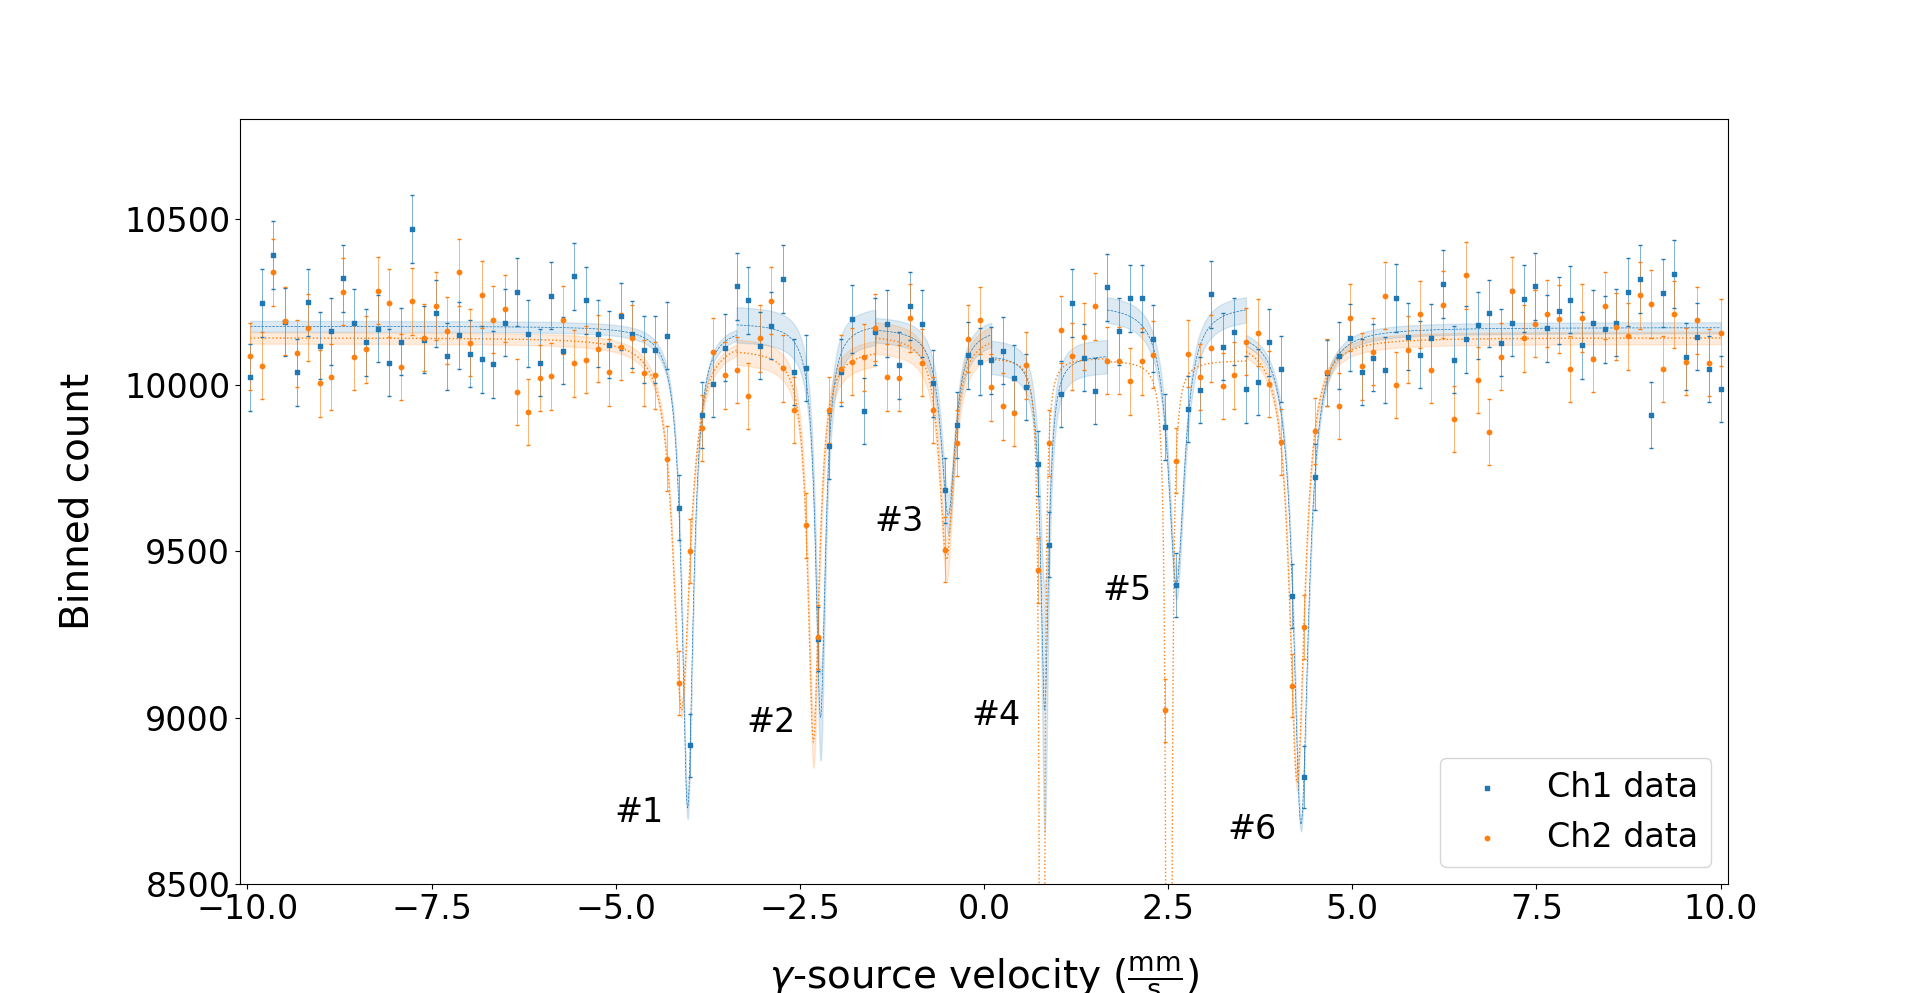
\includegraphics[width=1.0\textwidth]{./fig/Iron.png}
	\caption{Mössbauer spectrum of iron}{}\label{fig:iron}
\end{figure}

\begingroup
\renewcommand{\arraystretch}{1.3}
\begin{table}
	\begin{center}
	\caption{Mössbauer spectrum fit parameters for iron}
	\begin{tabular*}{0.9\textwidth}{@{\extracolsep{\fill}} c|ccccc}
  \toprule
	\hline
  Peak \# & $\Upphi_0$ & $A$ & $v_0$ & $\Gamma$ & Channel \\
	\hline
  \multirow{2}{*}{\#1} & $10177\pm16$ & $12\pm3.9$ & $-4.02\pm0.02$ & $0.184\pm0.043$ & Ch1 \\
  			               & $10142\pm17$ & $21\pm6.0$ & $-4.11\pm0.02$ & $0.277\pm0.049$ & Ch2 \\
  			                 \hline
  \multirow{2}{*}{\#2} & $10187\pm53$ & $8\pm6.2$ & $-2.22\pm0.03$ & $0.161\pm0.104$ & Ch1 \\
  			               & $10108\pm38$ & $10\pm5.6$ & $-2.32\pm0.01$ & $0.184\pm0.080$ & Ch2 \\
  			                 \hline
  \multirow{2}{*}{\#3} & $10173\pm37$ & $8\pm5.2$ & $-0.49\pm0.02$ & $0.234\pm0.099$ & Ch1 \\
  			               & $10151\pm47$ & $9\pm5.6$ & $-0.51\pm0.03$ & $0.235\pm0.076$ & Ch2 \\
  			                 \hline
  \multirow{2}{*}{\#4} & $10092\pm50$ & $4\pm6.0$ & $0.82\pm0.02$ & $0.130\pm0.193$ & Ch1 \\
  			               & $10082\pm65$ & $2\pm6.1$ & $0.79\pm0.05$ & $0.000\pm\infty$ & Ch2 \\
  			                 \hline
  \multirow{2}{*}{\#5} & $10243\pm38$ & $15\pm5.4$ & $2.61\pm0.02$ & $0.266\pm0.048$ & Ch1 \\
  			               & $10075\pm24$ & $3\pm2.4$ & $2.51\pm0.02$ & $0.000\pm\infty$ & Ch2 \\
  			                 \hline
  \multirow{2}{*}{\#6} & $10173\pm17$ & $23\pm5.1$ & $4.30\pm0.01$ & $0.246\pm0.036$ & Ch1 \\
  			               & $10142\pm19$ & $21\pm6.9$ & $4.25\pm0.01$ & $0.250\pm0.058$ & Ch2 \\
  			                 \hline
    \bottomrule
		\end{tabular*}
		\label{tab:iron}
	\end{center}

\end{table}
\endgroup


Due to the use of different emitter and absorber materials, a \textbf{isomer shift} occurs. This is caused by the different charge radii and electron distribution of the states involved in the transition.
 In the Mößbauer spectrum this results in a fixed shift of all absorption peaks around  the center (v=0), which overlaps with other phenomena. The isomer shift can be calculated by determining the center of gravity of pairwise connected lines. \\
At the $^{57}$Co-Rh source with natural iron as absorber an isomer shift of

\begin{equation}
\label{eq:isofe}
\Delta E = \SI{6.80 \pm 0.12}{\cdot 10^{-9} eV}
\end{equation}

occurs.

Another effect is the \textbf{hyper fine splitting} of $^{57}$Fe. This is caused by the movement of the shell electrons and a resulting magnetic field B at the location of the atomic nucleus.
Due to the Zeeman effect the degenerated state of the nucleus splits into $2I + $2 levels. I is the nuclear spin and there are $2I+1$ possible values of the magnetic quantum number m. The energy distances are given by

\begin{equation}
\label{eq:hyp1}
\Delta E_m = -\frac{m}{I} \mu B.
\end{equation}

It follows for energy of the $\gamma$-quanta with resonance absorption option considering the hyperfine splitting of excited (index a) and ground state (index g):

\begin{equation}
   E_{\gamma} = E_0 - \frac{m_a}{I_a}\mu_aB + \frac{m_g}{I_g}\mu_gB
\end{equation}

The excited state $I_a = \frac{3}{2}$ is split fourfold and the basic state $I_g =\frac{1}{2}$ is split twice.
For dipole transitions, however, the selection rule $\Delta m = m_a -m_g = 0\pm1$ applies, so only six transitions are permitted. The magnetic moment of the ground state is already known with

\begin{equation}
    \mu_g = \SI{0.0903\pm 0.0007}{\mu_k}
\end{equation}

where $\mu_k=\frac{e \hbar}{2m_p} $ corresponds to the nuclear magneton. Thus, the internal magnetic field and the magnetic moment of the excited state, $\mu_a$, can be determined.

The complete derivation of the calculation is in the blue book and is therefore only outlined here. The six possible transitions can be described by the newly defined sizes A, G and $I_0$. These are given by:
\begin{equation}
    A = \frac{\mu_aBc}{I_aE_0} \qquad
    G = \frac{\mu_gBc}{I_gE_0}
\end{equation}
where $I_0$ corresponds to the isomer shift already calculated. $E_0 =\SI{14.4\pm0.05}{\kilo eV}$ is the energy of the ground state and $c$ is the velocity of light. There are four cases to distinguish, depending on the relative size of the unknowns to each other. The case with the smallest deviation is chosen.

\begin{align*}
\text{(a)}& \quad v_1-2v_2-v_3=0 \\\
\text{(b)}& \quad v_1-2v_2+v_3=0 \\\
\text{(c)}& \quad v_1-v_2-2v_3=0 \\\
\text{(d)}& \quad -v_1+v_2+2v_3=0 \\\
\end{align*}

The velocities $v_1 >v_2 >v_3$ correspond to the positive absorption peaks of the Mößbauer spectrum and are already corrected for the isomer shift.

\begin{table}
    \centering
    \caption{Case distinction in the calculation of hyperfine structure splitting}
    \begin{tabular}{c c c}
    \toprule
         &Ch1 in $\SI{}{10^{-3}\frac{m}{s}}$ &Ch2 in $\SI{}{10^{-3}\frac{m}{s}}$  \\
         \hline
         $v_1$&4.16 &4.11 \\
         $v_2$&2.48&2.38 \\
         $v_3$&0.69&0.65 \\
         \hline
         $v_1-2v_2-v_3=0$&-1.47&-1.29\\
         $v_1-2v_2+v_3=0$&-0.10&0.01\\
         $v_1-v_2-2v_3=0$&0.32&0.44\\
         $-v_1+v_2+2v_3=0$&-0.32&-0.44\\



    \bottomrule
    \end{tabular}
    \label{tab:fe1}
\end{table}

The slightest deviation therefore occurred in case two (see $\autoref{tab:fe1}$). From this follows for the unknowns:
\begin{equation*}
    A = v_1-v_2 \qquad G = -v_2-v_3.
\end{equation*}
By transforming the equation follows:
\begin{equation}
    \mu_a =\frac{AI_aE_0}{Bc} = \frac{(v_1-v_2)I_aE_0}{Bc} \qquad B= \frac{GI_gE_0}{\mu_gc}=\frac{(-v_2-v_3)I_gE_0}{\mu_gc}
\end{equation}
where the magnetic field B is used in the first equation. Thus the inner magnetic field and the magnetic moment of the excited state are given by $\autoref{tab:fe2}$.
\\

\begin{table}
    \centering
    \caption{Inner magnetic field and magnetic moment of the excited $^{57}$Fe state.}

    \begin{tabular}{c c c c}
     \toprule
     &Ch1&Ch2&Mean \\
     \hline
     Inner magnetic field &  $-\SI{26.71\pm 0.39}{T}$ &$-\SI{25.54\pm 0.45}{T}$   &$-\SI{26.12\pm 0.71}{T}$ \\
     Magnetic moment& $-\SI{4.56\pm 0.15}{\cdot 10^{-9}eV}$  &$-\SI{4.91\pm 0.16}{\cdot 10^{-9}eV}$   &$-\SI{4.73\pm 0.23}{\cdot 10^{-9}eV}$\\
     \bottomrule
    \end{tabular}

    \label{tab:fe2}
\end{table}
